\section{Comunicazione tra elaboratori}
Il corso di reti di calcolatori si pone come obiettivo quello di risolvere il problema della \textbf{comunicazione tra computer}, inteso come il trasferimento di informazioni tra due o più sistemi, studiato in questo corso con un approccio \textbf{top-down}, ovvero a partire da un alto livello per andare sempre più a basso livello. In particolare, si presentano i due problemi fondamentali della comunicazione: \begin{itemize}
	\item \textbf{Protocollo di comunicazione}: Insieme di regole logiche che definiscono come le entità devono comunicare, nello specifico il \textbf{formato} dei messaggi, il loro \textbf{ordine} e le \textbf{azioni} da compiere alla loro ricezione.
	\item \textbf{Trasporto delle informazioni}: Il trasferimento fisico di dati fra due dispositivi. Richiede un'infrastruttura di rete composta da mezzi trasmissivi, come cavi o fibra ottica, dispositivi di rete e, naturalmente, protocolli di trasmissione.
\end{itemize}
\noindent Possiamo paragonare lo scambio di informazioni tra elaboratori con l'invio di una lettera. Il mittente scrive il messaggio, inserisce il foglio in una busta, con scritto l'indirizzo del destinatario e la consegna all'ufficio postale. Quest'ultimo la trasporterà fino al destinatario descritto, il quale potrà aprire la busta e leggere il contenuto del messaggio. Affinché il processo funzioni correttamente, è necessario seguire regole precise (quindi seguire il protocollo), come scrivere correttamente l'indirizzo del destinatario.\par
Nella pratica, la comunicazione tra due calcolatori avviene tramite una sequenza di livelli, spesso rappresentata come una pila verticale, dove ogni livello svolge una funzione specifica e prepara i dati per quello successivo. Intuitivamente: \begin{enumerate}
	\item L'applicazione genera il messaggio.
	\item Il messaggio è preparato per la trasmissione.
	\item I dati vengono inviati tramite la rete.
	\item Il destinatario riceve i dati.
	\item I dati sono elaborati fino a raggiungere l'applicazione finale.
\end{enumerate}
\begin{figure}[h]
	\centering
	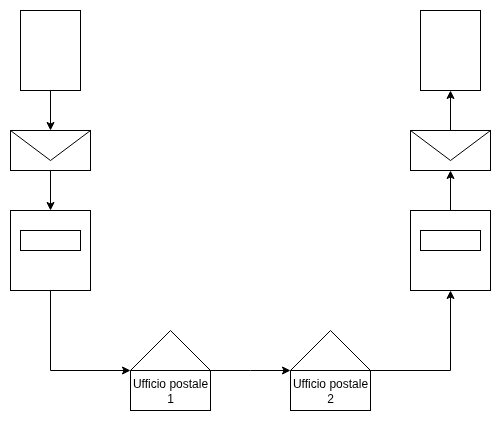
\includegraphics[width=0.7\linewidth]{Images/EsempioComunicazione.png}
	\caption{Esempio di comunicazione intuitivo}
	\label{fig:commExample}
\end{figure}
\noindent Naturalmente, lo scambio di informazioni non è unidirezionale, infatti si dice che il processo di trasferimento informazioni è \textbf{simmetrico} tra mittente e destinatario. Definiamo ora la struttura delle architetture di rete per capire in che modo comunichino gli elaboratori: possono avere elementi diversi, ma tutte presentano necessariamente gli \textbf{end-host}, ovvero i dispositivi per l'invio e ricezione di informazioni come computer o smartphone, gli \textbf{apparati di rete}, che permettono l'instradamento o la distribuzione dei dati nella rete, come router, switch e access point, e i \textbf{collegamenti}, i mezzi fisici o wireless che permettono la trasmissione dei dati, come fibra ottica o Wi-Fi.\par
Possiamo descrivere \textbf{Internet} in termini di infrastruttura di rete su scala globale, la quale fornisce servizi ad applicazioni distribuite. Per carpirne il funzionamento analizziamo un esempio su scala minore: le reti \textbf{Local Area Network} (LAN). Queste sono reti che coprono un'area limitata, come ad esempio un ufficio o una casa, dove sono presenti gli end-host. I principali dispositivi utilizzati sono: \begin{itemize}
	\item \textbf{Switch}: Dispositivo che collega fra loro più connessioni cablate.
	\item \textbf{Access point}: Dispositivo wireless che consente agli end-host di collegarsi alla rete.
\end{itemize}
\noindent Tipicamente lo switch rappresenta il punto centrale della rete cablata, mentre l'access point vi si collega per fornire connettività wireless. Nelle reti domestiche moderne è comune che router, switch e access point siano integrati nello stesso apparato.\par
Le LAN sono collegate alla rete Internet grazie ad un \textbf{router di bordo}, il quale, oltre al suddetto compito, è capace di inoltrare i dati ad altri router della rete globale, detta \textbf{backbone}, fino al raggiungimento di quello di destinazione, che consegnerà i dati all'end-host. 
\begin{figure}[h]
	\centering
	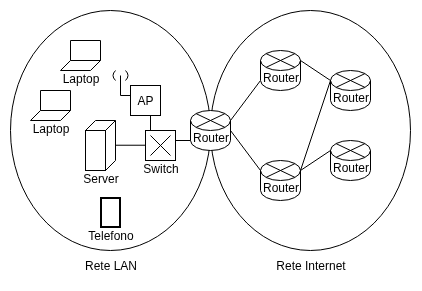
\includegraphics[width=0.8\linewidth]{Images/LAN-Internet connection.png}
	\caption{Collegamento tra rete LAN e Internet}
\end{figure}

\noindent La connettività Internet è fornita da organizzazioni chiamate \textbf{Internet Service Provider} (ISP), divise in tre livelli gerarchici: \begin{itemize}
	\item \textbf{Tier 1}: Operatori globali che gestiscono infrastrutture backbone internazionali.
	\item \textbf{Tier 2}: Operatori nazionali o regionali che acquistano connettività dai Tier-1 ma possono anche stabilire collegamenti diretti tra loro.
	\item \textbf{Tier 3}: Operatori locali che forniscono connettività agli utenti finali, come abitazioni, aziende, hotel.
\end{itemize}
\noindent In particolare, esistono gli \textbf{Autonomous Systems} (AS); insiemi di reti gestite da un'unica entità amministrativa e con una politica di routing comune.

%

\section{Commutazione di circuito e di pacchetto}
Ci sono due modalità principali per il trasferimento dei dati fra calcolatori: la \textbf{commutazione di circuito} e \textbf{di pacchetto}. La prima è stata storicamente usata nelle reti telefoniche tradizionali e ad oggi è nettamente meno diffusa. Il percorso tra la sorgente e la destinazione è allocato staticamente per la durata dello scambio dell'informazione, vedendo quindi le risorse di trasmissione dedicate alla comunicazione. Tuttavia, essendo la banda limitata, si può sostenere solo un certo numero di circuiti allo stesso tempo.\par
La gestione delle risorse avviene tramite il \textbf{Time Division Multiplexing}, una divisione delle risorse in slot da fornire ai vari utenti. Alternativamente si utilizza il \textbf{Frequency Division Multiplexing}, una divisione di spazio sulle frequenze sicché gli slot non interferiscano gli uni con gli altri, seguendo la logica della radio.
\begin{figure}[h]
	\centering
	\subcaptionbox{Commutazione di circuito}{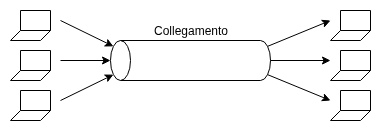
\includegraphics[width=0.45\linewidth]{Images/circuitComm.png}}
	\hfill
	\subcaptionbox{Grafico di commutazione}{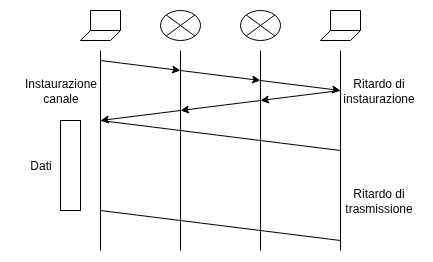
\includegraphics[width=0.5\linewidth]{Images/circuitCommGraph.png}}
\end{figure}

\noindent Questo sistema di commutazione ha due pro: \textbf{risorse dedicate} a ciascun utente, creando una comunicazione senza interruzioni o accodamento, e il \textbf{ritardo prevedibile} e costante dopo l'instaurazione del circuito. I problemi riguardano in primo luogo la \textbf{banda limitata}, poiché dando slot dedicati, in caso fossero tutti occupati, non sarebbe possibile usare il servizio. In secondo luogo parliamo di spreco delle risorse, perché, fintanto che rimane aperto, il canale è mantenuto attivo anche quando non si trasferiscono i dati.\newline

\noindent La \textbf{commutazione di pacchetto} invece vede i dati da trasferire divisi in sezioni indipendenti, a loro volta divise in due parti: l'\textbf{header}, contenente informazioni di controllo, tra cui indirizzo sorgente e destinazione, e la seconda, contenente i dati del pacchetto. Le varie sezioni sono inviate al router, il quale le accoda con un buffer per inviarle una alla volta passando per un bottleneck. Con questa metodologia è possibile gestire un numero molto elevato di utenti, poiché le risorse sono condivise dinamicamente. Infatti, non ci sono sprechi di risorse in caso un utente smetta di trasferire dati.\par
Il contro di questa modalità di commutazione è invece l'introduzione dei ritardi. I pacchetti si possono trasferire solo quando sono stati ricevuti tutti i relativi bit contenenti le informazioni tramite la modalità \textbf{store-and-forward switching}\footnote{Informazione salvata nel router, poi inoltrata a quello di destinazione.}. In particolare, è presente un ritardo iniziale legato al numero di apparati attraversati; smaltito questo, ci sarà quello di trasmissione. Un secondo problema è dato dalla potenziale \textbf{perdita di pacchetti}, perché in quanto i buffer hanno spazio limitato, può capitare di richiedere il trasferimento di pacchetti quando questo è pieno. In tal caso, il pacchetto viene scartato.
\begin{figure}[h]
	\centering
	\subcaptionbox{Commutazione di pacchetto}{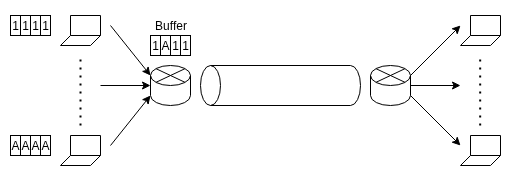
\includegraphics[width=0.45\linewidth]{Images/packageComm.png}}
	\hfill
	\subcaptionbox{Grafico di commutazione}{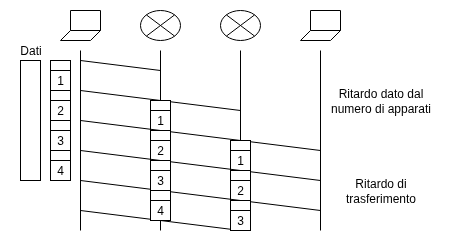
\includegraphics[width=0.5\linewidth]{Images/packageCommGraph.png}}
	\hfill
	\subcaptionbox{Divisione in pacchetti}{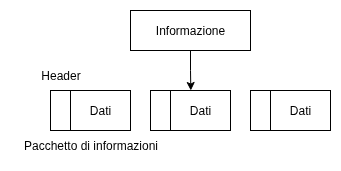
\includegraphics[width=0.5\linewidth]{Images/packageCommDivision.png}}
\end{figure}
\noindent Possiamo inoltre classificare i vari tipi di ritardo, valutando le cause fra ogni salto da un router all'altro: \begin{itemize}
	\item \textbf{Ritardo di elaborazione}: Legato all'architettura del router, è il tempo impiegato per l'elaborazione e invio del pacchetto.
	\item \textbf{Ritardo di accodamento}: Legato al buffer del link di uscita, in attesa che i dati siano trasmessi.
	\item \textbf{Ritardo di trasmissione}: Legato alla dimensione del pacchetto diviso la velocità di trasmissione: $d_{trans} = L/R$ Con $L$ dimensione del pacchetto in bit e $R$ velocità di trasmissione in bit al secondo.
	\item \textbf{Ritardo di propagazione}: Legato alla distanza da percorrere.
\end{itemize}
\noindent Normalmente il ritardo che incide di più è il secondo, perché può diventare dominante in caso di congestione. Inoltre possiamo considerare gli ordini di grandezza dei ritardi in base alla distanza. Generalmente valgono: \begin{itemize}
	\item \textbf{Comunicazione su stessa LAN}: $<1ms$
	\item \textbf{Comunicazione con stesso ISP}: $5-20ms$
	\item \textbf{Comunicazione su stesso continente}: $20-50ms$
	\item \textbf{Comunicazione intercontinentale}: $100-200ms$
\end{itemize}
\noindent Per ottenere il valore effettivo si usa il \textbf{ping}, il quale permette di misurare il \textbf{Round Trip Time}, ovvero il tempo di andata e ritorno di un messaggio fra due elaboratori.

%

\section{Modello di riferimento ISO-OSI e TCP/IP}